\documentclass{article}
\usepackage[utf8]{inputenc}
\usepackage[margin=1in]{geometry}

\usepackage{graphicx}
\usepackage{wrapfig}
\usepackage{algorithm}
\usepackage[noend]{algpseudocode}

\title{Eulerian Tours}
\author{Not Larry\footnote{Thanks to USACO training pages and TJIMO 2015!}}
\date{31 March 2017}

\begin{document}

\maketitle

\section{Introduction}

\begin{wrapfigure}{r}{0.3\textwidth}
  \vspace{-10pt}
  \begin{center}
    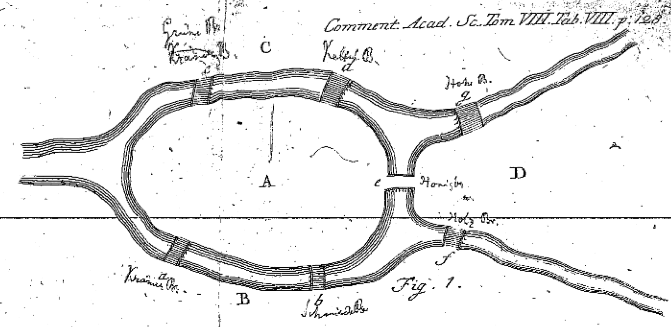
\includegraphics[width=0.3\textwidth]{bridges.png}
  \end{center}
  \vspace{0pt}
\end{wrapfigure}

%The \textbf{Seven Bridges of Königsberg} problem, posed by Euler in 

The port city of K\"{o}nigsberg in Prussia (now Kaliningrad, Russia) lies on two sides of a large river. In addition, there are two islands within the river also part of the city. As pictured, seven bridges connect the four land masses: Two from $A$ to $B$, two from $A$ to $C$, one from $A$ to $D$, one from $B$ to $D$, and one from $C$ to $D$.

Is it possible to walk through the city but cross every bridge exactly once? Euler famously solved this problem in 1736; this is his drawing of K\"{o}nigsberg, from his paper ``Solutio problematis ad geometriam situs pertinentis.''


\section{Eulerian tours and circuits}

\begin{wrapfigure}{r}{0.3\textwidth}
  \vspace{-40pt}
  \begin{center}
    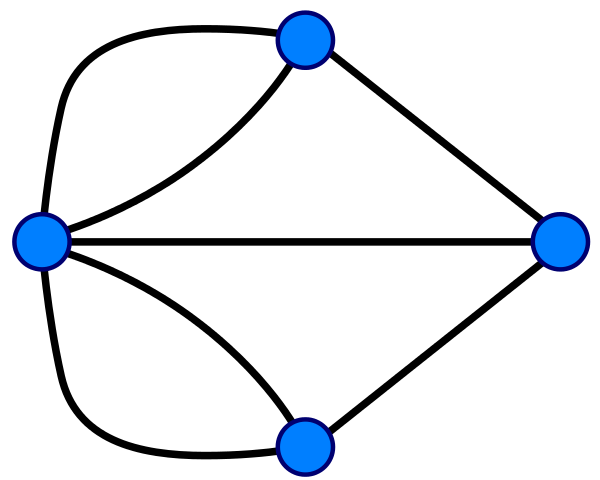
\includegraphics[width=0.25\textwidth]{Konigsberg_graph.png}
  \end{center}
  \vspace{0pt}
\end{wrapfigure}

The above problem reduces to the problem of finding an Eulerian tour in a graph. An \textbf{Eulerian tour} is a path which visits every edge in a graph exactly once. An \textbf{Eulerian circuit}, on the other hand, is such a path that starts and ends at the same vertex.

It turns out that the condition for determining whether an \textit{undirected} graph has an Eulerian tour or circuit is relatively simple. A precondition, of course, is that the graph must be connected --- we can't form an Eulerian tour if some edges are unreachable! In addition, we have the following conditions: 

\begin{enumerate}
    \item A graph has an Eulerian circuit if and only if every node has even degree.
    \item A graph has an Eulerian tour if and only if every node \textit{except for two} have even degree. Those two nodes must serve as the start and end points of the tour.
\end{enumerate}

Intuitively, we can understand this condition because we must leave a vertex the same number of times that we enter it. Otherwise, we'll either enter the vertex without leaving it, or vice versa. This means that, in fact, it is not possible to solve the Seven Bridges of K\"{o}nigsberg problem, as if we draw it as a graph, we see that all vertices have odd degree.

So far, we've only considered Eulerian tours in undirected graphs. In directed graphs, it is not as simple to determine whether a Eulerian tour exists. On the contrary, an Eulerian circuit exists in a directed graph if and only if the in-degree of every vertex is equal to its out-degree, which makes sense given our intuition above.

\newpage

\section{Finding an Eulerian tour}

The similar Hamiltonian path problem, a special case of the Traveling Salesman Problem, asks us to find a path that visits every vertex in the graph. Unfortunately, it is NP-complete. Fortunately, however, finding an Eulerian tour is much simpler! An algorithm to do so is outlined in pseudocode below.


\begin{algorithm}[H]
\caption{Finding an Eulerian tour}
\begin{algorithmic}

\State $circuit$ is an array

\Function{FindEulerCircuit}{}
    \State $circuit \gets$ empty array
    \State \Call{FindCircuit}{vertex $0$}
\EndFunction

\Function{FindCircuit}{vertex $u$}
    \While{vertex $u$ has neighbors}
        \State $v \gets$ an arbitrary neighbor of $u$
        \State delete edge between $u$ and $v$
        \State \Call{FindCircuit}{$v$}
    \EndWhile
    \State prepend $u$ to $circuit$
\EndFunction

\end{algorithmic}
\end{algorithm}


\section{Problems}

\begin{enumerate}
    \item \textbf{Tanya and Password} (Codeforces 508D)\\
    While dad was at work, a little girl Tanya decided to play with dad's password to his secret database. Dad's password is a string consisting of $n+2$ characters. She has written all the possible $n$ three-letter continuous substrings of the password on pieces of paper, one for each piece of paper, and threw the password out. Each three-letter substring was written the number of times it occurred in the password. Thus, Tanya ended up with $n$ pieces of paper.

    Then Tanya realized that dad will be upset to learn about her game and decided to restore the password or at least any string corresponding to the final set of three-letter strings. You have to help her in this difficult task. We know that dad's password consisted of lowercase and uppercase letters of the Latin alphabet and digits. Uppercase and lowercase letters of the Latin alphabet are considered distinct.
    
    \item \textbf{One-Way Reform} (Codeforces 723E)\\
    There are $n$ cities and $m$ two-way roads in Berland, each road connects two cities. It is known that there is no more than one road connecting each pair of cities, and there is no road which connects the city with itself. It is possible that there is no way to get from one city to some other city using only these roads.

    The road minister decided to make a reform in Berland and to orient all roads in the country, i.e. to make each road one-way. The minister wants to maximize the number of cities, for which the number of roads that begins in the city equals to the number of roads that ends in it.

\end{enumerate}

\end{document}
